\subsection{Procedimentos metodológicos} \label{subsec:metod}
   
    \subsubsection{Etapas da pesquisa}\label{subsubsec:etp}
    A pesquisa se deu seguindo as seguintes etapas:
    
    \begin{enumerate}[start=1, label = {\textbf{Etapa} \arabic* } ]
    	\item Análise exploratória dos dados – EDA (Exploratory Data Analysis) \label{etp:1}
    	\item O que vai ser usado como variáveis previsoras e qual será a variável a ser predita (MISO) \label{etp:2}
    	\item Fazer a decomposição STL (Seasonal-Trend Decomposition) Sazonalidade, Tendência e Resíduo \label{etp:3}
    	\item Divisão do conjunto de dados em treinamento, validação e teste 70\% para treinamento e validação e 30\% para teste, disso tirando dos 70\% e dividindo em 80\% para treinamento e 20\% para validação. Verificar a média e desvio padrão de cada um destes conjuntos de forma que obtenha a divisão mais adequada dos dados. \label{etp:4}
    	\item Estratégia de previsão (recursiva e iterada-método direto) \label{etp:5}
    	\item Horizonte de previsão (1 passo ou n passos a frente) \label{etp:6}
    	\item Modelos de previsão e métricas de desempenho \label{etp:7}
    	%\item Ajustar os hiperparâmetros dos modelos de previsão Hiperparâmetro ajusta a priori (ex: número de neurônios da rede neural), e parâmetro (pesos da rede neural) ajusta durante o processo. \label{etp:8}
    	\item Aplicar os modelos de previsão e fazer comparativo baseado em testes de significância estatística (\textit{Friedman e Nemenjy}) \label{etp:9}
    \end{enumerate}

\begin{figure}[H]
	\centering
	\caption{Mapa das Etapas}
	\label{fig:etapas}
	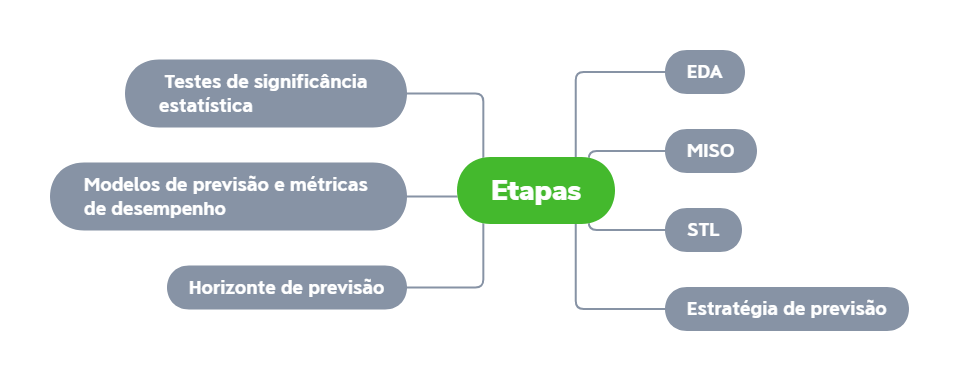
\includegraphics[width=1\linewidth]{Introducao/Figuras/Etapas}
	
	Fonte: Elaboração própria
\end{figure}




    